\documentclass{article}

%% Shamelessly adapted from a scribe template by Sanjeev Arora

%%%%%%%%%%%%%% Packages
% \usepackage[active,tightpage]{preview}
% \renewcommand{\PreviewBorder}{1in}
\usepackage[hidelinks]{hyperref}
\usepackage{amsmath,amssymb,amsthm,amstext,amsfonts,bbm,algorithm,algorithmicx,xspace,nicefrac,
  algpseudocode}
\usepackage{color,stmaryrd,enumerate,latexsym,bm,amsfonts,
  subfigure,wrapfig,verbatim,tabularx,textcomp}
\usepackage[small]{caption}
\usepackage{comment} 
\usepackage{epsfig} 
\usepackage{latexsym,nicefrac,bbm}
\usepackage{xspace}
\usepackage{color,fancybox,graphicx,url,subfigure}
\usepackage{enumitem, fullpage}
\usepackage{booktabs}
\usepackage{commath}
\usepackage{mdframed}
\usepackage{pdfsync}
\usepackage{tikz}
\usetikzlibrary {positioning}

%%%%%%%%%%%%%% Use for definitions
\newcommand{\defeq}{\stackrel{\textup{def}}{=}}

\DeclareMathOperator*{\argmax}{arg\,max}
\DeclareMathOperator*{\argmin}{arg\,min}

%%%%%%%%%%%%%% Theorem Environments
\newtheorem{theorem}{Theorem}[section]
\newtheorem{problem}[theorem]{Problem}
\newtheorem{lemma}[theorem]{Lemma}
\newtheorem{definition}[theorem]{Definition}
\newtheorem{corollary}[theorem]{Corollary}
\newtheorem{conjecture}[theorem]{Conjecture}
\newtheorem{proposition}[theorem]{Proposition}
\newtheorem{fact}[theorem]{Fact}
\newtheorem{remark}[theorem]{Remark}

%%%%%%%%%%%%%% Probability stuff
\DeclareMathOperator*{\pr}{\bf Pr}
\DeclareMathOperator*{\av}{\mathbbm{E}}
\DeclareMathOperator*{\var}{\bf Var}

%%%%%%%%%%%%%% Matrix stuff
\newcommand{\tr}[1]{\mathop{\mbox{Tr}}\left({#1}\right)}
\newcommand{\diag}[1]{{\bf Diag}\left({#1}\right)}

%% Notation for integers, natural numbers, reals, fractions, sets, cardinalities
%%and so on
\newcommand{\nfrac}[2]{\nicefrac{#1}{#2}}
\def\abs#1{\left| #1 \right|}
\renewcommand{\norm}[1]{\ensuremath{\left\lVert #1 \right\rVert}}

\newcommand{\floor}[1]{\left\lfloor\, {#1}\,\right\rfloor}
\newcommand{\ceil}[1]{\left\lceil\, {#1}\,\right\rceil}

\newcommand{\pair}[1]{\left\langle{#1}\right\rangle} %for inner product

\newcommand\B{\{0,1\}}      % boolean alphabet  use in math mode
\newcommand\bz{\mathbb Z}
\newcommand\nat{\mathbb N}
\newcommand\rea{\mathbb R}
\newcommand\com{\mathbb{C}}
\newcommand\plusminus{\{\pm 1\}}
\newcommand\Bs{\{0,1\}^*}   % B star use in math mode
\newcommand{\ones}{\mathbbm{1}}
\newcommand{\eye}{\mathbbm{I}}



\newcommand{\V}[1]{\mathbf{#1}\ignorespaces}
\renewcommand\AA{\boldsymbol{\mathit{A}}}
\newcommand\LL{\boldsymbol{\mathit{L}}}

% Used to denote bold commands
                                % e.g. vectors, matrices
\DeclareRobustCommand{\fracp}[2]{{#1 \overwithdelims()#2}}
\DeclareRobustCommand{\fracb}[2]{{#1 \overwithdelims[]#2}}
\newcommand{\marginlabel}[1]%
{\mbox{}\marginpar{\it{\raggedleft\hspace{0pt}#1}}}
\newcommand\card[1]{\left| #1 \right|} %cardinality of set S; usage \card{S}
\renewcommand\set[1]{\left\{#1\right\}} %usage \set{1,2,3,,}
\renewcommand\complement{\ensuremath{\mathsf{c}}}
\newcommand\poly{\mbox{poly}}  %usage \poly(n)
\newcommand{\comp}[1]{\overline{#1}}
\newcommand{\smallpair}[1]{\langle{#1}\rangle}
\newcommand{\ol}[1]{\ensuremath{\overline{#1}}\xspace}
\newcommand{\eps}{\epsilon}
\DeclareMathOperator{\vol}{\mathsf{vol}}


%%%%%%%%%%%%%% Mathcal shortcuts
\newcommand\calF{\mathcal{F}}
\newcommand\calP{\mathcal{P}}
\newcommand\calS{\mathcal{S}}
\newcommand\calG{\mathcal{G}}
\newcommand\calH{\mathcal{H}}
\newcommand\calC{\mathcal{C}}
\newcommand\calD{\mathcal{D}}
\newcommand\calI{\mathcal{I}}
\newcommand\calV{\mathcal{V}}
\newcommand\calK{\mathcal{K}}
\newcommand\calN{\mathcal{N}}
\newcommand\calX{\mathcal{X}}
\newcommand\calU{\mathcal{U}}
\newcommand\calE{\mathcal{E}}
\newcommand\calL{\mathcal{L}}
\newcommand\calR{\mathcal{R}}


%%%%%%%%%%%%%% {{{ authornotes }}}
\definecolor{Mygray}{gray}{0.8}

 \ifcsname ifcommentflag\endcsname\else
  \expandafter\let\csname ifcommentflag\expandafter\endcsname
                  \csname iffalse\endcsname
\fi

\ifnum\showauthornotes=1
\newcommand{\todo}[1]{\colorbox{Mygray}{\color{red}#1}}
\else
\newcommand{\todo}[1]{#1}
\fi

\ifnum\showauthornotes=1
\newcommand{\Authornote}[2]{{\sf\small\color{red}{[#1: #2]}}}
\newcommand{\Authoredit}[2]{{\sf\small\color{red}{[#1]}\color{blue}{#2}}}
\newcommand{\Authorcomment}[2]{{\sf \small\color{gray}{[#1: #2]}}}
\newcommand{\Authorfnote}[2]{\footnote{\color{red}{#1: #2}}}
\newcommand{\Authorfixme}[1]{\Authornote{#1}{\textbf{??}}}
\newcommand{\Authormarginmark}[1]{\marginpar{\textcolor{red}{\fbox{%\Large
#1:!}}}}
\else
\newcommand{\Authornote}[2]{}
\newcommand{\Authoredit}[2]{}
\newcommand{\Authorcomment}[2]{}
\newcommand{\Authorfnote}[2]{}
\newcommand{\Authorfixme}[1]{}
\newcommand{\Authormarginmark}[1]{}
\fi


%%%%%%%%%%%%%% Logical operators
\newcommand\true{\mbox{\sc True}}
\newcommand\false{\mbox{\sc False}}
\def\scand{\mbox{\sc and}}
\def\scor{\mbox{\sc or}}
\def\scnot{\mbox{\sc not}}
\def\scyes{\mbox{\sc yes}}
\def\scno{\mbox{\sc no}}

%% Parantheses
\newcommand{\paren}[1]{\unskip\left({#1}\right)}
\newcommand{\sqparen}[1]{\unskip\left[{#1}\right]}
\newcommand{\curlyparen}[1]{\unskip\left\{{#1}\right\}}
\newcommand{\smallparen}[1]{\unskip({#1})}
\newcommand{\smallsqparen}[1]{\unskip[{#1}]}
\newcommand{\smallcurlyparen}[1]{\unskip\{{#1}\}}

%% short-hands for relational simbols

\newcommand{\from}{:}
\newcommand\xor{\oplus}
\newcommand\bigxor{\bigoplus}
\newcommand{\logred}{\leq_{\log}}
\def\iff{\Leftrightarrow}
\def\implies{\Rightarrow}

%--------------------------------------------------------------------------------------------------------------------------------
% Optimization macros
%--------------------------------------------------------------------------------------------------------------------------------
%\providecommand{\argmax}{\mathop\mathrm{arg max}} % Defining math symbols
%\providecommand{\argmin}{\mathop\mathrm{arg min}}
\providecommand{\arccos}{\mathop\mathrm{arccos}}
\providecommand{\dom}{\mathop\mathrm{dom}}
\providecommand{\diag}{\mathop\mathrm{diag}}
\providecommand{\tr}{\mathop\mathrm{tr}}
%\providecommand{\abs}{\mathop\mathrm{abs}}
\providecommand{\card}{\mathop\mathrm{card}}
\providecommand{\sign}{\mathop\mathrm{sign}}
\providecommand{\conv}{\mathop\mathrm{conv}} % Convex hull
\def\rank#1{\mathrm{rank}({#1})}
\def\supp#1{\mathrm{supp}({#1})}

\providecommand{\minimize}{\mathop\mathrm{minimize}}
\providecommand{\maximize}{\mathop\mathrm{maximize}}
\providecommand{\subjectto}{\mathop\mathrm{subject\;to}}

%\renewcommand\eqref[1]{Eq.~(\ref{#1})}

\def\openright#1#2{\left[{#1}, {#2}\right)}

%--------------------------------------------------------------------------------------------------------------------------------
% Vectors and matrices
%--------------------------------------------------------------------------------------------------------------------------------
\newcommand{\boldone}{\mbf{1}} % Bold 1
\newcommand{\ident}{\mbf{I}} % Identity matrix
% \def\v#1{\mbi{#1}} % Vector notation
%\def\norm#1{\left\|{#1}\right\|} % A norm with 1 argument
\newcommand{\onenorm}[1]{\norm{#1}_1} % L1 norm
\newcommand{\twonorm}[1]{\norm{#1}_2} % L2 norm
\newcommand{\infnorm}[1]{\norm{#1}_{\infty}} % Linfty norm
\newcommand{\opnorm}[1]{\norm{#1}_{\text{op}}} % Operator norm
\newcommand{\fronorm}[1]{\norm{#1}_{\text{F}}} % Frobenius norm
\newcommand{\nucnorm}[1]{\norm{#1}_{*}} % Frobenius norm
\def\staticnorm#1{\|{#1}\|} % A static norm that does not resize with input
\newcommand{\statictwonorm}[1]{\staticnorm{#1}_2} % L2 norm
\newcommand{\inner}[1]{{\langle #1 \rangle}} % inner product
\newcommand{\binner}[2]{\left\langle{#1},{#2}\right\rangle} % Inner product with expandable brackets
\def\what#1{\widehat{#1}}

\def\twovec#1#2{\left[\begin{array}{c}{#1} \\ {#2}\end{array}\right]}
\def\threevec#1#2#3{\left[\begin{array}{c}{#1} \\ {#2} \\ {#3} \end{array}\right]}
\def\nvec#1#2#3{\left[\begin{array}{c}{#1} \\ {#2} \\ \vdots \\ {#3}\end{array}\right]} % An n-vector with three arguments
\DeclareMathOperator\spn{span}


%% macros to write pseudo-code

\newlength{\pgmtab}  %  \pgmtab is the width of each tab in the
\setlength{\pgmtab}{1em}  %  program environment
 \newenvironment{program}{\renewcommand{\baselinestretch}{1}%
\begin{tabbing}\hspace{0em}\=\hspace{0em}\=%
\hspace{\pgmtab}\=\hspace{\pgmtab}\=\hspace{\pgmtab}\=\hspace{\pgmtab}\=%
\hspace{\pgmtab}\=\hspace{\pgmtab}\=\hspace{\pgmtab}\=\hspace{\pgmtab}\=%
\+\+\kill}{\end{tabbing}\renewcommand{\baselinestretch}{\intl}}
\newcommand {\BEGIN}{{\bf begin\ }}
\newcommand {\ELSE}{{\bf else\ }}
\newcommand {\IF}{{\bf if\ }}
\newcommand {\FOR}{{\bf for\ }}
\newcommand {\TO}{{\bf to\ }}
\newcommand {\DO}{{\bf do\ }}
\newcommand {\WHILE}{{\bf while\ }}
\newcommand {\ACCEPT}{{\bf accept}}
\newcommand {\REJECT}{\mbox{\bf reject}}
\newcommand {\THEN}{\mbox{\bf then\ }}
\newcommand {\END}{{\bf end}}
\newcommand {\RETURN}{\mbox{\bf return\ }}
\newcommand {\HALT}{\mbox{\bf halt}}
\newcommand {\REPEAT}{\mbox{\bf repeat\ }}
\newcommand {\UNTIL}{\mbox{\bf until\ }}
\newcommand {\TRUE}{\mbox{\bf true\ }}
\newcommand {\FALSE}{\mbox{\bf false\ }}
\newcommand {\FORALL}{\mbox{\bf for all\ }}
\newcommand {\DOWNTO}{\mbox{\bf down to\ }}

% Theorem-type environments
% \theoremstyle{break} 
% \theoremheaderfont{\scshape}
% \theorembodyfont{\slshape}
% \newtheorem{Thm}{Theorem}[section]
% \newtheorem{Lem}[Thm]{Lemma}
% \newtheorem{Cor}[Thm]{Corollary}
% \newtheorem{Prop}[Thm]{Proposition}
% % \theoremstyle{plain} 
% % \theorembodyfont{\rmfamily} 
% \newtheorem{Ex}[Thm]{Exercise}
% \newtheorem{Exa}[Thm]{Example}
% \newtheorem{Rem}[Thm]{Remark}
% % \theorembodyfont{\itshape}
% \newtheorem{Def}[Thm]{Definition}
% \newtheorem{Conj}[Thm]{Conjecture}
% \newtheorem{Obs}[Thm]{Observation}
% \newtheorem{Ques}[Thm]{Question}
%\newenvironment{proof}{\noindent {\sc Proof:}}{$\Box$ \medskip} 
\newenvironment{problems} % Definition of problems
 {\renewcommand{\labelenumi}{\S\theenumi}
	\begin{enumerate}}{\end{enumerate}}


%%%%%%%%%%%%%%%%% Proof Environments

\def\FullBox{\hbox{\vrule width 6pt height 6pt depth 0pt}}
%
%\def\qed{\ifmmode\qquad\FullBox\else{\unskip\nobreak\hfil
%\penalty50\hskip1em\null\nobreak\hfil\FullBox
%\parfillskip=0pt\finalhyphendemerits=0\endgraf}\fi}

\def\qedsketch{\ifmmode\Box\else{\unskip\nobreak\hfil
\penalty50\hskip1em\null\nobreak\hfil$\Box$
\parfillskip=0pt\finalhyphendemerits=0\endgraf}\fi}

%\newenvironment{proof}{\begin{trivlist} \item {\bf Proof:~~}}
 %  {\qed\end{trivlist}}

\newenvironment{proofsketch}{\begin{trivlist} \item {\bf
Proof Sketch:~~}}
  {\qedsketch\end{trivlist}}

\newenvironment{proofof}[1]{\begin{trivlist} \item {\bf Proof
#1:~~}}
  {\qed\end{trivlist}}

\newenvironment{claimproof}{\begin{quotation} \noindent
{\bf Proof of claim:~~}}{\qedsketch\end{quotation}}


%%%%%%%%%%%%%%%%%%%%%%%%%%%%%%%%%%%%%%%%%%%%%%%%%%%%%%%%%%%%%%%%%%%%%%%%%%%
%%%%%%%%%%%%%%%%%%%%%%%%%%%%%%%%%%%%%%%%%%%%%%%%%%%%%%%%%%%%%%%%%%%%%%%%%%%




\newlength{\tpush}
\setlength{\tpush}{2\headheight}
\addtolength{\tpush}{\headsep}

\newcommand{\handout}[5]{
   \noindent
   \begin{center}
   \framebox{ \vbox{ \hbox to \textwidth { {\bf \coursenum\ :\  \coursename} \hfill #5 }
       \vspace{3mm}
       \hbox to \textwidth { {\Large \hfill #2  \hfill} }
       \vspace{1mm}
       \hbox to \textwidth { {\it #3 \hfill #4} }
     }
   }
   \end{center}
   \vspace*{4mm}
   \newcommand{\lecturenum}{#1}
   \addcontentsline{toc}{chapter}{Lecture #1 -- #2}
}

\newcommand{\lecturetitle}[4]{\handout{#1}{#2}{Lecturer: \courseprof
  }{Scribes: #3}{Date: #4}}
\newcommand{\guestlecturetitle}[5]{\handout{#1}{#2}{Lecturer:
    #4}{Scribe: #3}{Lecture #1 - #5}}


%%%%%%%%%%%%%%%%%%%%%%%%%%%%%%%%%%%%%%%%%%%%%%%%%%%%%%%%%
%%% Commands to include figures


%% PSfigure

\newcommand{\PSfigure}[3]{\begin{figure}[t] 
  \centerline{\vbox to #2 {\vfil \psfig{figure=#1.eps,height=#2} }} 
  \caption{#3}\label{#1} 
  \end{figure}} 
\newcommand{\twoPSfigures}[5]{\begin{figure*}[t]
  \centerline{%
    \hfil
    \begin{tabular}{c}
        \vbox to #3 {\vfil\psfig{figure=#1.eps,height=#3}} \\ (a)
    \end{tabular}
    \hfil\hfil\hfil
    \begin{tabular}{c}
        \vbox to #3 {\vfil\psfig{figure=#2.eps,height=#3}} \\ (b)
    \end{tabular}
    \hfil}
  \caption{#4}
  \label{#5}
%  \sublabel{#1}{(a)}
%  \sublabel{#2}{(b)}
  \end{figure*}}

\newcounter{fignum}

% fig
%command to insert figure. usage \fig{name}{h}{caption}
%where name.eps is the postscript file and h is the height in inches
%The figure is can be referred to using \ref{name}
\newcommand{\fig}[3]{%
\begin{minipage}{\textwidth}
\centering\epsfig{file=#1.eps,height=#2}
\caption{#3} \label{#1}
\end{minipage}
}%


% ffigure
% Usage: \ffigure{name of file}{height}{caption}{label}
\newcommand{\ffigure}[4]{\begin{figure} 
  \centerline{\vbox to #2 {\hfil \psfig{figure=#1.eps,height=#2} }} 
  \caption{#3}\label{#4} 
  \end{figure}} 

% ffigureh
% Usage: \ffigureh{name of file}{height}{caption}{label}
\newcommand{\ffigureh}[4]{\begin{figure}[!h] 
  \centerline{\vbox to #2 {\vfil \psfig{figure=#1.eps,height=#2} }} 
  \caption{#3}\label{#4} 
  \end{figure}} 


% {{{ draftbox }}}
\ifnum\showdraftbox=1
\newcommand{\draftbox}{\begin{center}
  \fbox{%
    \begin{minipage}{2in}%
      \begin{center}%
%        \begin{Large}%
          \large\textsc{Working Draft}\\%
%        \end{Large}\\
        Please do not distribute%
      \end{center}%
    \end{minipage}%
  }%
\end{center}
\vspace{0.2cm}}
\else
\newcommand{\draftbox}{}
\fi


%% Complexity classes
\newcommand\p{\mbox{\bf P}\xspace}
\newcommand\np{\mbox{\bf NP}\xspace}
\newcommand\cnp{\mbox{\bf coNP}\xspace}
\newcommand\sigmatwo{\mbox{\bf $\Sigma_2$}\xspace}
\newcommand\ppoly{\mbox{\bf $\p_{\bf /poly}$}\xspace}
\newcommand\sigmathree{\mbox{\bf $\Sigma_3$}\xspace}
\newcommand\pitwo{\mbox{\bf $\Pi_2$}\xspace}
\newcommand\rp{\mbox{\bf RP}\xspace}
\newcommand\zpp{\mbox{\bf ZPP}\xspace}
\newcommand\bpp{\mbox{\bf BPP}\xspace}
\newcommand\ph{\mbox{\bf PH}\xspace}
\newcommand\pspace{\mbox{\bf PSPACE}\xspace}
\newcommand\npspace{\mbox{\bf NPSPACE}\xspace}
\newcommand\dl{\mbox{\bf L}\xspace}
\newcommand\ma{\mbox{\bf MA}\xspace}
\newcommand\am{\mbox{\bf AM}\xspace}
\newcommand\nl{\mbox{\bf NL}\xspace}
\newcommand\conl{\mbox{\bf coNL}\xspace}
\newcommand\sharpp{\mbox{\#{\bf P}}\xspace}
\newcommand\parityp{\mbox{$\oplus$ {\bf P}}\xspace}
\newcommand\ip{\mbox{\bf IP}\xspace}
\newcommand\pcp{\mbox{\bf PCP}}
\newcommand\dtime{\mbox{\bf DTIME}}
\newcommand\ntime{\mbox{\bf NTIME}}
\newcommand\dspace{\mbox{\bf SPACE}\xspace}
\newcommand\nspace{\mbox{\bf NSPACE}\xspace}
\newcommand\cnspace{\mbox{\bf coNSPACE}\xspace}
\newcommand\exptime{\mbox{\bf EXP}\xspace}
\newcommand\nexptime{\mbox{\bf NEXP}\xspace}
\newcommand\genclass{\mbox{$\cal C$}\xspace}
\newcommand\cogenclass{\mbox{\bf co$\cal C$}\xspace}
\newcommand\size{\mbox{\bf SIZE}\xspace}
\newcommand\sig{\mathbf \Sigma}
\newcommand\pip{\mathbf \Pi}

%%Computational problems
\newcommand\sat{\mbox{SAT}\xspace}
\newcommand\tsat{\mbox{3SAT}\xspace}
\newcommand\tqbf{\mbox{TQBF}\xspace}

\addbibresource{refs.bib}

\begin{document}
\begin{center}
    \Large{Derandomization and Nearly Logarithmic Space Laplcian Solvers}

    \vspace{1em}

    \large{Devansh Shringi, Harry Sha}
    \vspace{1em}

    \large{CSC2240 Final Report - Fall 2022}
    \vspace{2em}
\end{center}  

\section{Context: Space Bounded Complexity}
\subsection{L, RL, NL}
An essential resource for computation is space. Like in the time-bounded computation, we can define several interesting complexity classes. The following are analogs for $P, RP$, and $NP$, but restricted to logarithmic space instead of polynomial time. Let $n$ be the length of the input.

\begin{definition}[L]
    $L$ is the set of decision problems decidable by a \textbf{deterministic} Turing Machine using at most $O(\log(n))$ cells on the work tape.
\end{definition}


\begin{definition}[RL]
    $NL$ is the set of decision problems decidable by a \textbf{probabilistic} Turing Machine with one-sided error using at most $O(\log(n))$ cells on the work tape.
\end{definition}

\begin{definition}[NL]
    $NL$ is the set of decision problems decidable by a \textbf{non-deterministic} Turing Machine using at most $O(\log(n))$ cells on the work tape.
\end{definition}

The classes are summarized in the following table.
\begin{figure}[ht]
    \begin{center}
    \begin{tabular}{l|l|l}
    & $x \in L$  & $x \notin L$ \\ \hline
    $L$   & 1          & 0            \\
    $RL$  & $\geq 2/3$ & 0            \\
    $NL$  & $> 0$      & 0           
    \end{tabular}
    \caption{Acceptance Probabilities}
    \end{center}
\end{figure}

In this view, it is straightforward to see $L \subset RL \subset NL$. However, just as in the poly-time complexity setting, it is unknown whether or not these containments are strict.


\begin{open-problem}Is $L$ equal to $RL$? Is $RL$ equal to $NL$?
\end{open-problem}

The current conjecture is that $L = RL$ but $L \neq NL$. If $L = RL$, then it would mean that we could \textbf{derandomize} any randomized algorithm that runs in logarithmic space using logarithmic space. Thus, the derandomization we'll study here provides some limited evidence for $L = RL$. 

\subsection{Connectivity}

Define the following decision problems:
\begin{align*}
STCON &= \left\{ \ab{G, s, t} : G \text{ is a \textbf{directed} graph and there is a path from $s$ to $t$ in  G}\right\}\\
USTCON &= \left\{ \ab{G, s, t} : G \text{ is an \textbf{undirected} graph and there is a path from $s$ to $t$ in  G}\right\}
\end{align*}
\begin{fact}
    $\STCON$ is complete for $NL$. I.e., $\STCON \in NL$ and $\STCON$ is hard for $NL$ with respect to logspace reductions.
\end{fact}

It is currently unknown if $\STCON \in RL$. However, there is a very natural \textit{randomized} logspace algorithm for $\USTCON$, i.e., $\USTCON \in RL$. In fact, a simple random walk, \Cref{alg:randomwalk}, does the job.
\begin{algorithm}[ht]
    \caption{Random Walk}
    \KwIn{$G, s, t$}
    $c = s$\;
    \For{$n^4$ times}{
        \If{$c = t$}{
            \KwRet{True}
        }
        $c \from \Gamma(c)$
    }
    \KwRet{False}
    \caption{Random Walk}\label{alg:randomwalk}
\end{algorithm}

The random walk uses at most logarithmic space since you only keep track of a single vertex, requiring $\log(n)$ bits to identify.  \cite{aleliunasRandomWalksUniversal1979}, showed that if $s$ and $t$ are indeed connected by an undirected path, then this algorithm returns true with high probability, so this is indeed an $RL$ algorithm for $\USTCON$.

\subsection{Solving Laplacian System}

In the later half of this report, we will focus on finding solution for the following equation for a graph $G$ on $n$ vertices and given $b\in \mathbb{R}^n$

$$\LL x=b$$

where $\LL$ denotes the Laplacian matrix of the graph. The Laplacian of a graph is the matrix $\LL=\boldsymbol{\mathit{D}}-\AA$ where $\boldsymbol{\mathit{D}}$ is a diagonal matrix $n\times n$ with weighted degree of $v$ as the $(v,v)$ entry and $\AA$ is the adjacency matrix. It can also be seen that solving a Laplacian system allows you to solve connectivity in undirected setting, and therefore is at least as hard as USTCON, and so is interesting if it can be done in $L$. Solving the directed case of Laplacian also implies $RL=L$. The solution for the undirected case in \cite{peng2014efficient} used random sampling and was later found to have a solution running in deterministic logspace, using derandomized squaring in \cite{murtaghDerandomizationConnectivityUndirected2017}. Thus, this also further supports the argument of $RL=L$.

As we saw in class, solving Laplacian systems has applications in various parts of complexity and algorithms, calculating Effective Resistance, finding Max Flow, Sampling Spanning Trees, and Graph Sparsification being a few.



\section{Derandomization of The Random Walk}
In a breakthrough result, \cite{reingoldUndirectedConnectivityLogspace2005} showed that this algorithm could be derandomized - i.e., that $\USTCON \in L$. We will present a proof by \cite{rozenmanDerandomizedSquaringGraphs2005}. 


\subsection{Intuition}
The idea of the proof is to improve the connectivity of $G$, so much so that if $s$ and $t$ are connected, they are connected by an edge and then examine the neighbors of $s$. The measure of connectivity we will use is expansion.

\subsection{Technicalities}
\paragraph{Regularlity.} First, to make our lives easier, we'll assume that all graphs are regular. To do so, replace a single vertex, $v$, with a cycle of length $\deg(v)$ such that each vertex in the cycle is adjacent to one of $v$'s neighbors. Then, we can add a self-loop to each vertex. Thus, without loss of generality, it suffices to consider input graphs that are $4$-regular and contains a loop on each vertex.

\paragraph{Labelling.} A consistent labeling of a $K$-regular directed graph is an assignment of edges to $[K]$ such that for each vertex, all the outgoing edges have unique labels, and all the incoming edges have unique labels. For a vertex $v$ and an edge label $i \in [K]$, let $v[i]$ be the neighbor of $v$ on the edge labeled $i$.

We'll also assume that all the graphs we work with have a consistent labeling and that all operations preserve the consistent labeling (you can check this yourself!).

\subsection{Notation}
For any integer $N$,
\begin{itemize}
    \item $I_N$ is the $N \times N$ identity matrix,
    \item $J_N$ is the $N \times N$ matrix with each entry equal $1/N$,
    \item $\1_N$ is the $N \times 1$ all ones matrix, and 
    \item $u_N = \frac{1}{N}\1_N$ is the uniform distribution on $[N]$.
\end{itemize}

\subsection{Expansion}

\begin{definition}[Expander]
    Let $X$ be a $K$-regular graph on $N$ vertices with random walk matrix $M$. $X$ is called an $(N, K, \lambda)$-expander if the second largest (in absolute value) of $M$, denoted $\lambda(X)$, is at most $\lambda$.

    Using the fact that $M$ is real and symmetric, we know that the eigenvectors of the $M$ are orthogonal, and by the Courant-Fisher Theorem, 

    $$
    \lambda(X) = \max_{v \perp \1} \frac{\|Mv\|}{\|v\|}
    $$
\end{definition}

\textbf{Intuition}. $\lambda \in [0,1]$, and the smaller $\lambda(X)$ is, the better the connectivity of the graph and the faster the convergence of a random walk to the uniform distribution.

Another useful characterization of $(N, D, \lambda)$ graphs is the following
\begin{lemma}\label{lem:expander-characterization}
    Let $M$ be the transition matrix of a $K$-regular graph on $N$ vertices. 

    $$
\lambda(M) \leq \lambda \iff M = (1 - \lambda)J_N + \lambda C
    $$
    for some matrix $C$ with $\|C\| \leq 1$.
\end{lemma}

The following lemma relates the expansion of a graph and the diameter.

\begin{lemma} \label{lem:high-expansion}
    Let $X$ be a $(N, D, \frac{1}{2N^{1.5}})$-expander. Then $X$ contains a pair between any pair of vertices. The probability that a random neighbor of $v$ is equal $w$ is at least $\frac{1}{N} - \frac{1}{N^2} > 0$.
\end{lemma}

Thus, when the expansion of a graph is very small, it contains a clique.

\begin{proof}
    For a given vertex, $v$, the distribution of random neighbors is $Me_v$. I.e., the probability that a random neighbor of $v$ equals $w$ is $(Me_v)_w$. Thus, we want to show that every entry of $Me_v$ is at least $\frac{1}{N} - \frac{1}{N^2}$. To do so, we'd like to use expansion, so we will transform $e_v$ into one that is orthogonal to $\1$. Let $u = \frac{1}{N}\1$ be the uniform distribution on vertices. We'll consider $e_v - u$. This has several nice properties:
    \begin{enumerate}
        \item $e_v - u$ is orthogonal to $\1$.
        \item $Mu = u$, so every element of $Me_v \geq \frac{1}{N} - \frac{1}{N^2}$ iff every element of $M(e_v - u)$ has is value at least $-\frac{1}{N^2}$. Clearly, it is sufficient to show that every element of $M(e_v - u)$ has absolute value at most $\frac{1}{N^2}$.
        \item $\|e_v - u\| = \sqrt{(N-1)\frac{1}{N^2} + \frac{(N-1)^2}{N^2}} \leq 2$
    \end{enumerate}
    Thus, since the expansion is at most $\frac{1}{2N^{1.5}}$, $\|M(e_v - u)\|^2 \leq \frac{1}{N^3}$. Let $m$ be the smallest element of $M(e_v - u)$ in absolute value. Then, $\|M(e_v - u)\|^2 \geq Nm^2$. Putting the two together, we get $m \leq \frac{1}{N^2}$ as required.
    
\end{proof}


The following fact shows that all regular graphs have some expansion to start with - the goal will be to reduce this down to the value in \Cref{lem:high-expansion}.

\begin{lemma}\label{lem:starting-expansion}
    Let $X$ be a $D$-regular graph on $N$ vertices with a loop on each vertex. Then $\lambda(X) \leq 1 - \frac{1}{2D^2N^2}$
\end{lemma}

\subsection{Squaring}

\begin{definition}[Squaring]
    Let $X$ be a graph with adjacency matrix $A$. Then, the square of $X$ denoted $X^2$ is the graph with adjacent matrix $A^2$. I.e., if there is a path of length $2$ from $u$ to $v$ in $X$, there is now an edge from $u$ to $v$.
\end{definition}

\begin{remark}
One can also view the square as placing a clique on the neighborhood of each vertex. For example, see \Cref{fig:square}.
\end{remark}

\begin{figure}
    \begin{center}
        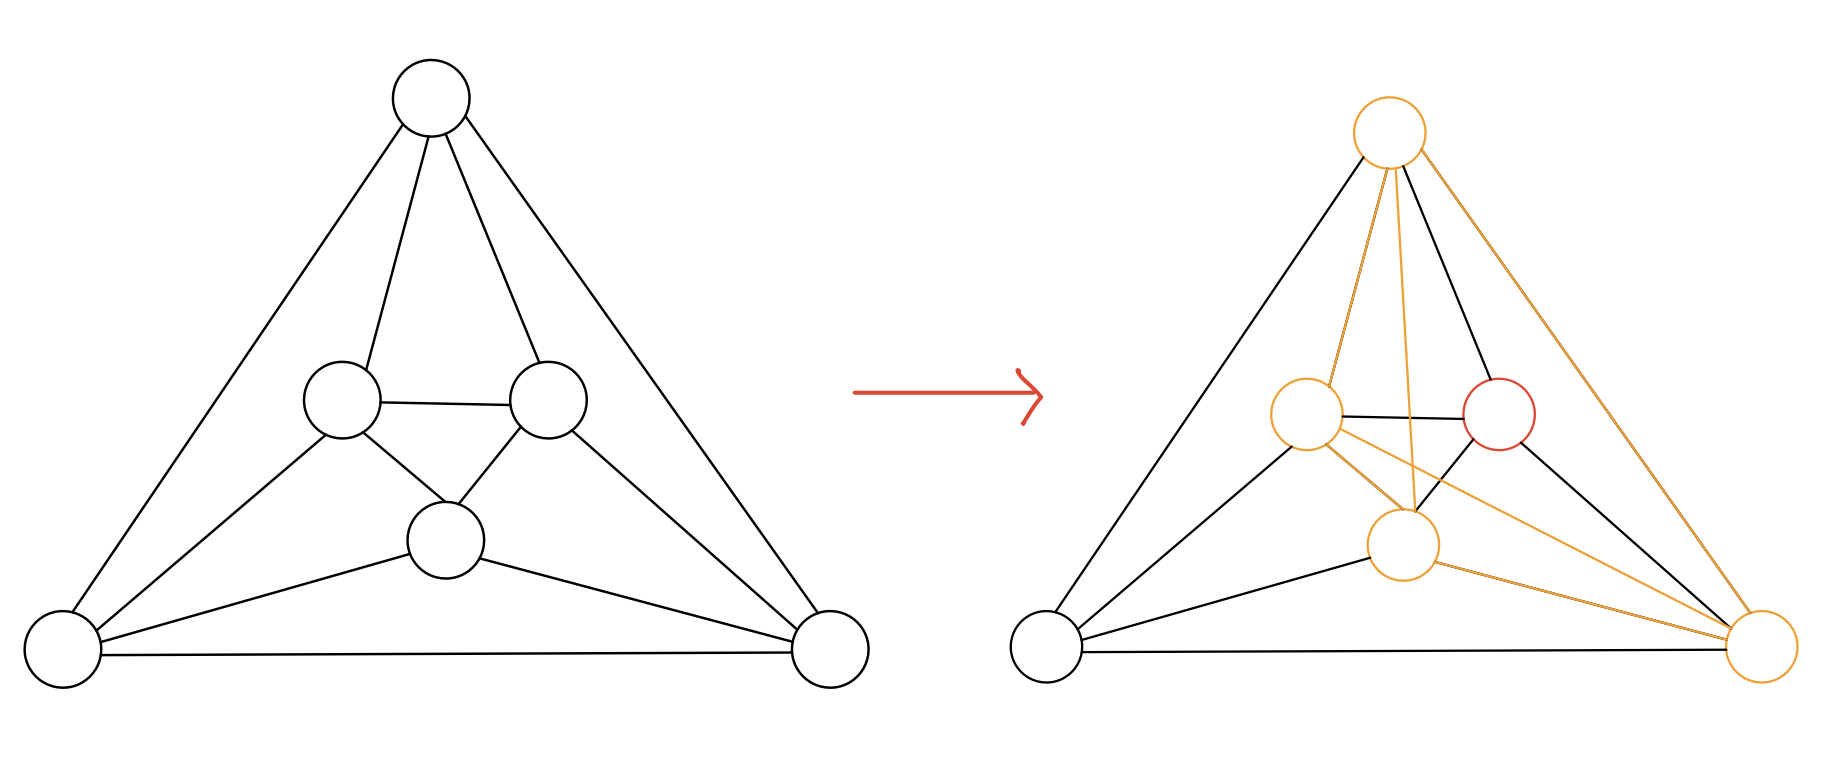
\includegraphics[width=0.8\textwidth]{square.png}
    \end{center}
    \caption{Placing a clique on the neighborhood of a vertex}\label{fig:square}
\end{figure}


\begin{remark}
Since the transition matrix simply squares, the $\lambda(X^2) = \lambda(X)^2$, so the expansion squares (making it smaller than before).    
\end{remark}

The downside of this operation is that the degree also squares - if $X$ was $D$-regular, $X$ is now $D^2$-regular. To ameliorate this, instead of placing a clique on every neighborhood, place an auxiliary graph (with fewer edges), thereby adding only a subset of the paths of length two in $X$. This is the definition of the derandomized square.

\subsection{Derandomized Squaring}
\begin{definition}[Derandomized Square \cite{rozenmanDerandomizedSquaringGraphs2005}]
    Let $X$ be a labeled $K$-regular graph on the vertex set $[N]$, and let $G$ be a $D$-regular graph on the vertex set $[K]$, the derandomized square, denoted $X \dsquare G$ has vertex set $[N]$ and is $KD$ regular. For $a \in [K]$, and $b \in [D]$, the $(a, b)$th neighbor of $v$ is the $(v[a])[a[b]]$. 
\end{definition}

Note $a[b] \in [K]$ and is viewed as an edge label for $v[a]$. The edge $(a, b)$ captures the path of length two $v \to v[a] \to v[a][a[b]]$. See \Cref{dsquare}.

\begin{figure}
    \begin{center}
        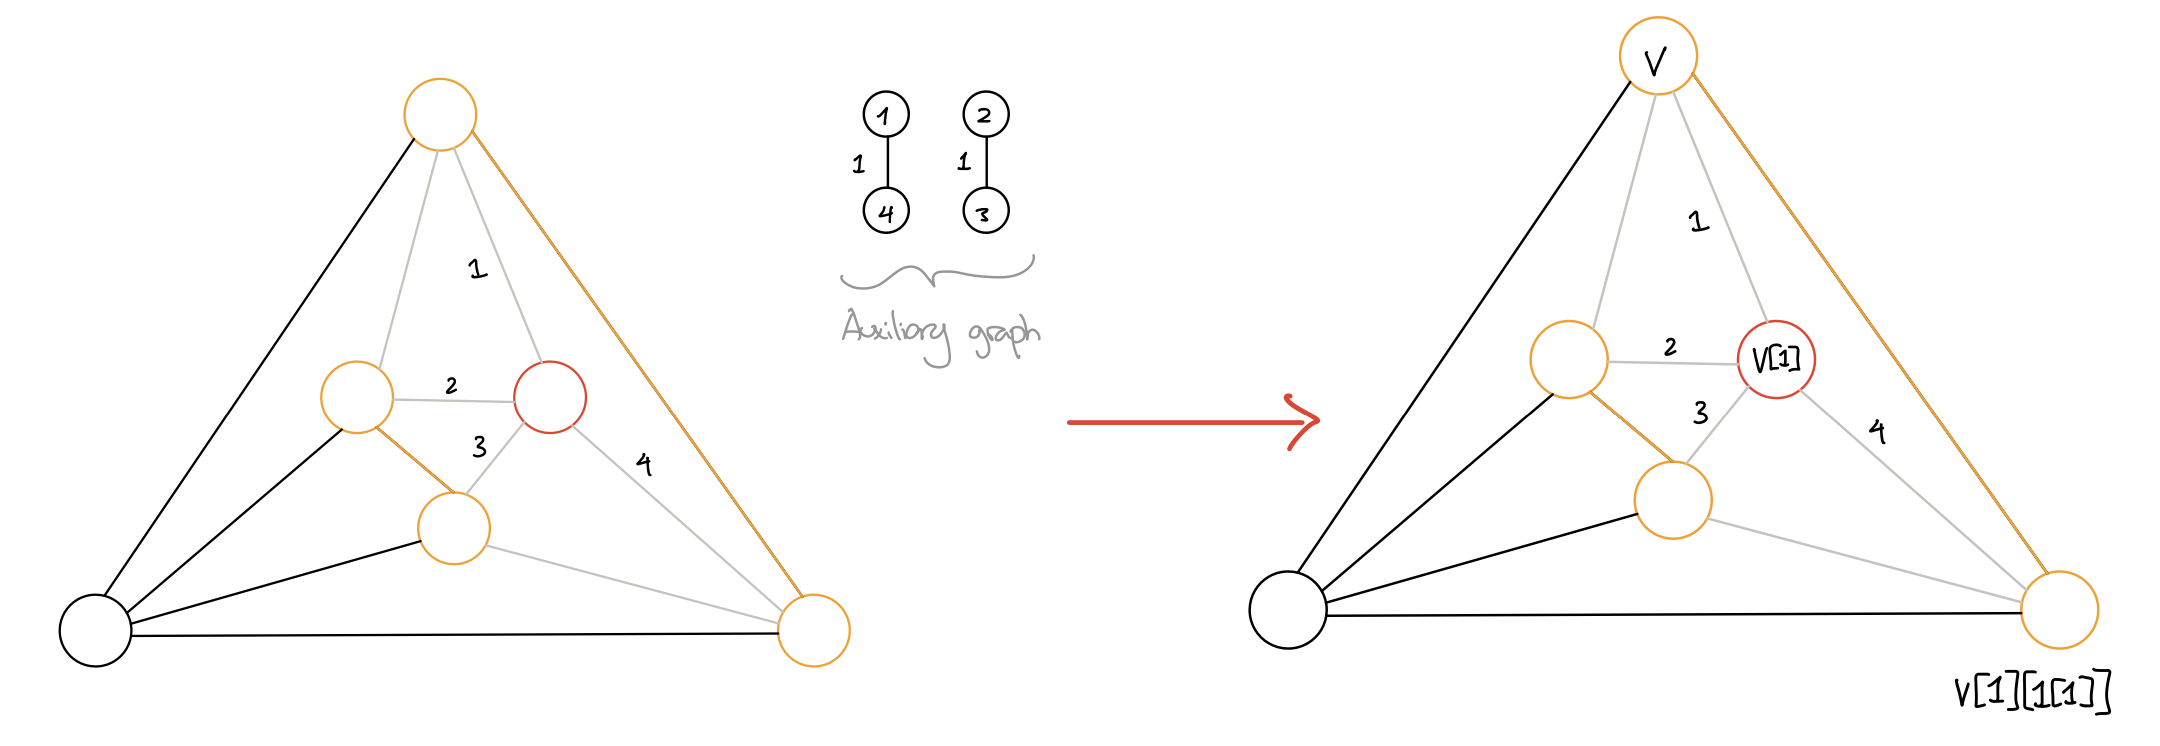
\includegraphics[width=0.9\textwidth]{dsquare.png}
    \end{center}
    \caption{Placing an auxiliary graph on the neighborhood of a vertex. Shows the (1,1)th neighbor of $v$.}\label{dsquare}
\end{figure}


\begin{lemma}[Derandomized Square is almost as good as Squaring \cite{rozenmanDerandomizedSquaringGraphs2005}]\label{lem:dsquare-expansion}
    If $X$ is a consistently labelled $(N, K, \lambda)$-graph and $G$ is a $(K, D, \mu)$-graph, then $X \dsquare G$ is an $(N, KD^2, f(\lambda, \mu))$-graph, where 
    $$
    f(\lambda, \mu) = \lambda^2 + \mu - \lambda^2\mu
    $$
\end{lemma}

\begin{remark}
$f(\lambda, \mu) \leq \lambda^2 + \mu$
\end{remark}

By the remark, we see that the derandomized square has expansion close to the regular square when $\mu$ is small (that is, when $G$, the auxiliary graph, is also a good expander). This crucial fact makes the derandomized square useful - it has expansion almost as good as the square but smaller degree.

\begin{proof}[Proof of \Cref{lem:dsquare-expansion}]
    Let $M$ be the transition matrix of $X\dsquare G$. We'll show that any vector perpendicular to $\1$ shrinks by a factor of at least $f(\lambda, \mu)$. The proof will bound the matrix norm of $M$. Let $A$ be the transition matrix of $X$ and $B$ be the transition matrix of $G$.

    To define the $M$, it will be useful to consider a random step on $X \dsquare G$. Recall that the $(a, b)$th neighbor of $u$ for $a \in [K], b \in [D]$, is the $a[b]$th neighbor of $u[a]$. For a random step in $X \dsquare G$ starting at $u$, think of it as happening in the following process.
    \begin{enumerate}
        \item Sample $a \from [K]$. Move to state $(u, a)$.
        \item Go to state $(u[a], a)$.
        \item Sample $b \from \Gamma(a)$. Go to $(u[a], b)$.
        \item Go to $(u[a][b], b)$.
        \item Output $u[a][b]$.
    \end{enumerate}


    To encode the states algebraically, we'll use the tensor product - i.e., $u \otimes v$ encodes $(u, v)$. The transformations that take each state to the next are illustrated in \Cref{fig:sequence}.

    \begin{figure}[ht]
        \begin{center}
            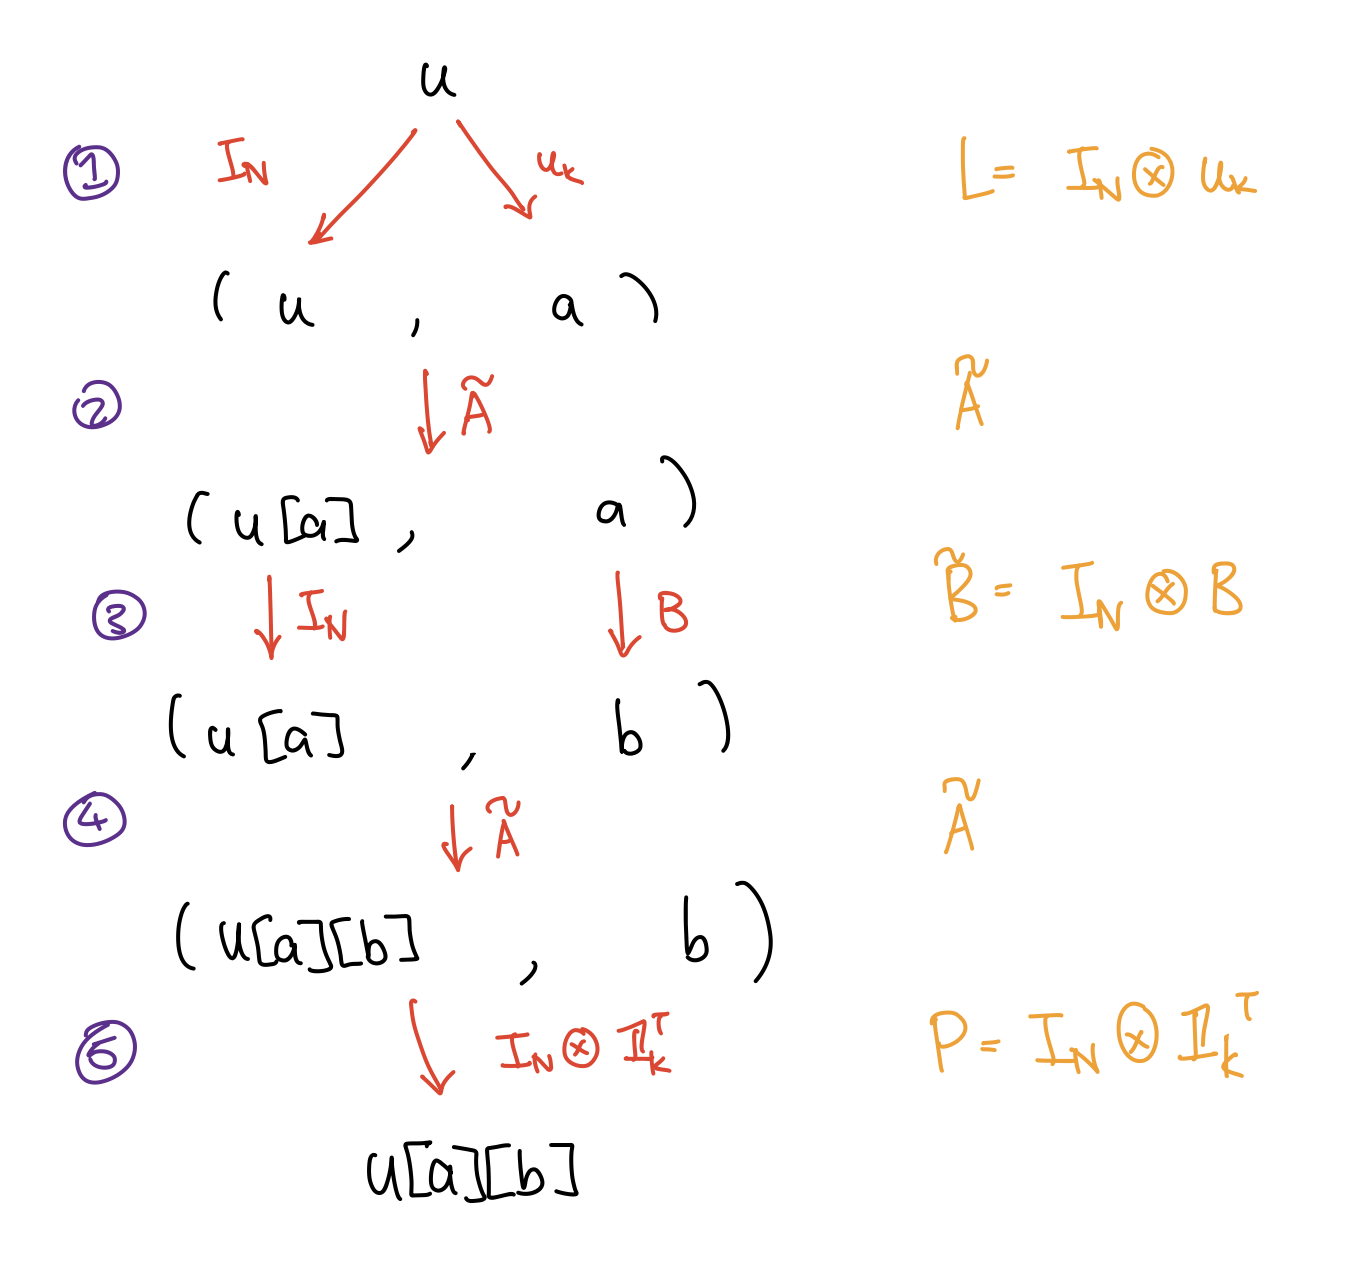
\includegraphics[width=0.7\textwidth]{equations.png}
        \end{center}
        \caption{Sequence of transformations} \label{fig:sequence}
    \end{figure}
    
    The first step corresponds to mapping $L = I_N \otimes u_K$. This makes a vector $u$ to $(u, u_K)$. For step, 2, we apply a permutation matrix $\tilde{A}$ such that $\tilde{A}_{(u, a), (u', a')}$ is $1$ iff $a' = a$, and $u' = u[a]$. Note that this fixes the second coordinate and moves the first coordinate according to the second. In the third step, we fix the first coordinate and go to a random neighbor of $a$ in $G$, which corresponds to applying the identity to the first coordinate and the random walk matrix of $G$ to the second. This is captured by the matrix $\tilde{B} = I_N \otimes B$. Step 4  applies $\tilde{A}$ again. Finally, step $5$ sums up all the possible ways we could have reached $u[a][b]$. This corresponds to a linear map $P = I_N \otimes \1_K^T$ that projects from probability distributions on $[N] \times [K]$ to probability distributions on $[N]$.

    Altogether, we have $$M = P\tilde{A}\tilde{B}\tilde{A}L.$$

    Using \Cref{lem:expander-characterization}, we can decompose $B = (1 - \mu)J_K + \mu C$ where $||C|| \leq 1$. Thus, $\tilde{B} = (1 - \mu)(I_N \otimes J_K) + \mu(I_N \otimes C) = (1 - \mu)(I_N \otimes J_K) + \mu\tilde{C}$. Substituting this back into the definition of $M$, we have 
    \begin{align*}
        M = (1 - \mu)P\tilde{A}(I_N \otimes J_K)\tilde{A}L + \mu P\tilde{A}\tilde{C}\tilde{A}L.
    \end{align*}


    For the first term, note that $LP = (I_N \times u_k) (I_N \times 1_k^T) = I_N \otimes J_K$. Additionally, note that $P\tilde{A}L = A$ Thus, $P\tilde{A}(I_N \otimes J_K)\tilde{A}L = A^2$, and has norm at most $\lambda^2$. For the second, note that $\|L\| = K^{-1/2}$, $\|P\| = K^{1/2}$, $||\tilde{A}|| = 1$ (since $\tilde{A}$ is a permutation matrix), and $\|\tilde{C}\| \leq 1$. Therefore, $\left\|P\tilde{A}\tilde{C}\tilde{A}L\right\| \leq 1$. Thus, we can write 
    $$
    M = (1 - \mu)A^2 + \mu D
    $$
    Hence for a vector $v \perp \1_N$, we have 
    \begin{align*}
        \|Mv\| \leq (1 - \mu)\|A^2v\| + \mu\|Dv\| = (\lambda^2 + \mu - \lambda^2\mu)\|v\|,
    \end{align*}
    as required.

\end{proof}


\subsection{Sketch of the rest of the proof}
Here is an outline of the rest of the proof
\begin{itemize}
    \item Assume the input graph is $4$-regular with a self-loop on each vertex.
    \item Such a graph starts with some expansion by \Cref{lem:starting-expansion}
    \item Iteratively shrink the expansion using the derandomized square with a sequence of carefully chosen auxiliary graphs and applying \Cref{lem:dsquare-expansion}.
    \item Repeat until the expansion is small enough that we can apply \Cref{lem:high-expansion}, and argue that the degree is still small enough to do this in logarithmic space.
\end{itemize}


\section{Solving Laplacians in Small Space}

For a $d$-regular undirected multigraph $G$ on $n$ vertices, we will be using $\MM=\frac{1}{d}A$ to denote the $n \times n$ transition matrix for the random walk on $G$. Normalized Laplacian of such a graph $G$ is defined as

$$\LL(G)=\II-\MM(G)$$ 

And the target of our report is to find a solution for the following equation.

$$\LL x=b$$

From class, we learned that it is equivalent to finding the Moore-Penrose pseudo-inverse of $\LL$ denoted by $\LL^{+}$, which is an inverse of $\LL$ in all space except the kernel of $\LL$.

It can be shown that using a Laplacian solver in an undirected graph, we can solve for $st$-connectivity in the undirected graph. We saw in previous sections how undirected connectivity is in $L$, and therefore it is a natural question to ask if we can solve the tougher problem of finding solution to Laplacian equations also in $L$. It should also be noted that creating a Directed Laplacian solver working in LogSpace will show $RL=L$.

\subsection{Peng-Spielman Solver}

Before we look at the solution for undirected Laplacian in LogSpace in \cite{murtaghDerandomizationConnectivityUndirected2017}, we will look at the solution known previously given in \cite{peng2014efficient}, and why it doesn't work in $L$. 

If we have a simplifying assumption that $\LL^+=\LL^{-1}$, we can look at a simple solution like

$$\LL^{-1}=\frac{1}{\II-\MM}=\sum_{i=0}^\infty \MM^i=\prod_{k=0}^\infty(\II+\MM^{2^k})$$

and we can get a simple solution if we truncate the product at a suitable $k$. As all eigenvalues of $\MM$ are $\leq 1$, the higher terms contribute less and thus can be approximated. But this identity doesn't work well under spectral approximation, so Peng-Spielman use the following identity in this lemma.

\begin{lemma}\label{identity}
    For a graph $G$, with random walk transition matrix $\MM$, Laplacian $\LL$ and $\JJ$ being the matrix with all entries $\frac{1}{n}$, we have
    $$\LL(G)^{+}=\frac{1}{2}\cdot(\II-\JJ+(\II+\MM(G))\LL(G^2)^+(\II+\MM(G)))$$
\end{lemma}

\begin{proof}
    The idea is to show that LHS and RHS have the same eigenvalues and eigenvectors. Let $\Psi_1=\V{1},\ldots,\Psi_n$ be the orthonormal eigenvectors of $\LL$ with eigenvalues $0,\gamma_2,\ldots,\gamma_n$. We know we can write $\LL$ as $\sum_{i=1}^n\gamma_i\Psi_i\Psi_i^\top$. Similarly, we have $\LL^+=\sum_{i=2}^n\frac{1}{\gamma_i}\Psi_i\Psi_i^\top$.

    Consider $\Psi_i$ for $i\neq 1$, and therefore $\Gamma_i\neq 0$. $\Psi_i$ will also be an eigenvector for $\II$($\II\Psi_i=\Psi_i$) with eigenvalue $1$. It will also be an eigenvector for $\MM=\II-\LL$ ($\MM\Psi_i=\II\Psi_i-\LL\Psi_i=(1-\gamma_i)\Psi_i$) with eigenvalue $(1-\gamma_i)$. As we have $\LL^+=\sum_{i=2}^n\frac{1}{\gamma_i}\Psi_i\Psi_i^\top$, we have RHS multiplied with $\Psi_i$ as
    
    $$\LL^+\Psi_i=\left(\sum_{j=2}^n\frac{1}{\gamma_j}\Psi_j\Psi_j^\top\right)\Psi_i=\frac{1}{\gamma_i}\Psi_i\Psi_i^\top\Psi_i=\frac{1}{\gamma_i}\Psi_i$$
    
    It similarly will also be an eigenvector of $\MM^2$($(1-\gamma_i)^2$ eigenvalue) and $\II-\MM^2$($1-(1-\gamma_i)^2$ eigenvalue). Using the definition of Pseudoinverse above, it will also be eigenvector of $\LL(G^2)^+$ with eigenvalue $\frac{1}{1-(1-\gamma_i)^2}$. Finally, as we know $\Psi_i$ is orthogonal to $\V{1}$, we have $\Psi_i$ as eigenvector of $\JJ$($\JJ\Psi_i=0$) with eigenvalue $0$. So multiplying LHS with $\Psi_i$ we see

    \begin{align*}
    \frac{1}{2}\cdot(\II-\JJ+(\II+\MM(G))\LL(G^2)^+(\II+\MM(G)))\Psi_i&=\frac{1}{2}\left(1-0+(1+1-\gamma_i)\frac{1}{1-(1-\gamma_i)^2}(1+1-\gamma_i)\right)\Psi_i\\
    &=\frac{1}{2}\cdot\left(1+\frac{2-\gamma_i}{\gamma_i}\right)\Psi_i \\
    &=\frac{1}{\gamma_i}\Psi_i    
    \end{align*}

    Therefore, $\Psi_i$ is an eigenvector for both LHS and RHS with eigenvalue $\frac{1}{\gamma_i}$, and this is true for all $i\neq 1$. 

    For eigenvector $\V{1}$, we see that it is an eigenvector for $\II,\JJ,\MM$ with eigenvalue $1$. For $\LL^{+}\V{1}$ we know it be $0$ as all $\Psi_i$ are orthonormal to $\V{1}$. Therefore, $\V{1}$ is eigenvector of LHS with eigenvalue $0$. We also know $\MM^2\V{1}=1$, and therefore $\LL(G^2)\V{1}=\LL^+(G)^2\V{1}=0$. So we see for RHS multiplied with $\V{1}$

    \begin{align*}
    \frac{1}{2}\cdot(\II-\JJ+(\II+\MM(G))\LL(G^2)^+(\II+\MM(G)))\V{1}&=\frac{1}{2}\left(1-1+(1+1)0(1+1)\right)\V{1}\\
    &=0  
    \end{align*}

    Thus, LHS and RHS both have $\V{1}$ as eigenvector with eigenvalue 0. Thus, LHS and RHS have all $n$ eigenvectors and eigenvalues same, and therefore are equal.
\end{proof}

This identity works well under spectral approximation, and thus it's computation can be truncated after $O(\log n)$ iteration of recursion, as we know $\LL^+(G^{2^{\log n}})=\LL^+(G^{2^n})\approx\LL^+(\KK_n)=\II-\JJ$.

The problem with repeating the recursion several times is that the degree grows very fast $d^{2^k}$ after $k$ steps, and thus the computation is not feasible.

Peng-Spielman solve this issue using the spectral sparsifiers of \cite{spielman2011spectral} we studied in class. In every step, you replace $G^2$ with a sparsified version of it that retains $\frac{\Tilde{O}(n)}{\epsilon^2}$ edges giving $G'$ such that $L(G')\approx_{\epsilon} L(G^2)$. We can easily see in the proof of Lemma \ref{identity} that replacing $\LL^+(G^2)$ with $\LL^+(G')$ will give an $\epsilon$ spectral approximation of $\LL^+(G)$. Since, we repeat these steps $O(\log n)$ times, the final error in $\LL^+(G_0)$ will be $\epsilon\cdot\log n$ and therefore to keep it constant, we will use $\epsilon=\frac{1}{O(\log n)}$ for constant error approximation, which will keep the number of edges at $\Tilde{O}(n)$ and thus computation at each level can be done efficiently.\\
\\

\textbf{Problems wrt LogSpace Computation}\\
The main 2 problems that prevent this solution from working in LogSpace are the following:

\begin{enumerate}
    \item Spectral Sparisifier as we studied in class require random sampling, which cannot be used if we require an algorithm that runs in deterministic LogSpace.
    \item In the above computation, even if each level of computation can be done to use $\Tilde{O}(\log n)$ space, as there are $O(\log n)$ levels of recursive computation, the total space used will be $O(\log^2 n)$.
\end{enumerate}

To get a solution in $L$, both these problems need to be solved, and we will use derandomized squaring similar to what we saw earlier for the USTCON problem.

\subsection{Using Derandomized Squaring}

As we saw in the case of USTCON, we can replace $G^2$ with derandomized square of $G$ with an expander $H$, denoted by $G\dsquare H$, and have spectral properties remain the same while ensuring the  degree doesn't blow up too quickly. This was used in \cite{murtaghDerandomizationConnectivityUndirected2017} to give a Laplacian solver using $\Tilde{O}(\log n)$ space. 

Therefore, the idea will be to replace $\LL(G^2)^+$ with $\LL(G\dsquare H)^+$, where $H$ is a $c$-regular graph on $d$-vertices with absolute value of second-largest eigenvalue $\epsilon$. First, we show that $\LL(G\dsquare H)$ will be an $\epsilon$ approximation of $\LL(G^2)$, and hence it can be used in identity.

\begin{lemma}\label{spec-approx}
    $$\LL(G^2)\approx_{\epsilon}\LL(G\dsquare H)$$
\end{lemma}
\begin{proof}
    As discussed in proof of \ref{lem:dsquare-expansion}, we have that 
    $$\MM(G\dsquare H)= P\tilde{A}\tilde{B}\tilde{A}L$$

    Recall from the proof that we have $PL=\II_n$ and $LP=\II_{n\cdot d}\otimes \JJ=\II_n\otimes \JJ_d$, and $\Tilde{A}$ is a symmetric $(n\cdot d)\times (n\cdot d)$ matrix with property $\Tilde{A}^2=\II_n$. Since, $H$ is an $\epsilon$ expander, we have that $\LL_H\approx_\epsilon\LL_{K_d}$ where $K_d$ denotes the clique on $d$-vertices. As $B$ was the transition matrix for $H$, we have $\LL_H=\II-B$, and $\II_{n}\otimes \LL_H=\II_{n\cdot d}-\Tilde{B}$. We also have $\MM(G)=P\Tilde{A}L$

    So we start with 

    $$\LL(G\dsquare H)=\II_n-\MM(G\dsquare H)$$

    Using the above identities, we can write $\II_n$ as $P\tilde{A}\II_{n\cdot d}\tilde{A}L$, while we know $\MM(G\dsquare H)= P\tilde{A}\tilde{B}\tilde{A}L$. Therefore, we have

    \begin{align*}
        \LL(G\dsquare H)&=P\tilde{A}\II_{n\cdot d}\tilde{A}L-P\tilde{A}\tilde{B}\tilde{A}L\\
        &=P\tilde{A}(\II_{n\cdot d}-\tilde{B})\tilde{A}L\\
        &=P\tilde{A}(\II_{n}\otimes \LL_H)\tilde{A}L
    \end{align*}

    As we have $\LL_H\approx_\epsilon\LL_K$, we can replace $\II_{n}\otimes \LL_H$ with $\II_{n}\otimes \LL_K$ approximately. Also, we know $\LL_K=\II_d-\JJ_d$, so $\II_{n}\otimes \LL_K=\II_n\otimes \II_d-\II_n\otimes\JJ_d=\II_{n\cdot d}-LP$. Therefore, we have


    \begin{align*}
        \LL(G\dsquare H)&=P\tilde{A}(\II_{n}\otimes \LL_H)\tilde{A}L\\
        &\approx_\epsilon P\tilde{A}(\II_{n}\otimes \LL_K)\tilde{A}L\\
        &=P\tilde{A}(\II_{n\cdot d}-\II_n\otimes\JJ_d)\tilde{A}L\\
        &=P\tilde{A}\II_{n\cdot d}\tilde{A}L-P\tilde{A}(\II_n\otimes\JJ_d)\tilde{A}L\\
        &=\II_n-P\tilde{A}LP\tilde{A}L\\
        &=\II_n-(\MM(G))^2\\
        &=\II_n-\MM(G^2)\\
        &=\LL(G^2)
    \end{align*}

    Therefore, we have $\LL(G^2)\approx_{\epsilon}\LL(G\dsquare H)$.\\
\end{proof}

\textbf{Sequence of Derandomized Square}

We start with $G_0=G$ as our original graph. We use a sequence of $c$-regular Expanders $H_0,H_1,\cdots,H_k$ for $k$ derandomized squares and use of Lemma \ref{identity}. $H_i$ is an $\epsilon$-expander on $d\cdot c^{i}$ vertices. WE define $G_{i+1}$ as follows

$$G_{i+1}=G_i\dsquare H_{i}$$

It is easy to see that $G_{i}$ is a $d\cdot c^{i}$-regular multigraph on $n$ vertices. We go up to $k=O(\log n)$ iterations, at which points $G_k\approx K_n$ and $\LL_{G_k}\approx \II-\JJ$. To prevent the degree from growing exponentially, so that we can do the computations in logspace, we choose $c=poly(\log n)$ and therefore all degree remain small. We also have the new version of Lemma \ref{identity}, which we use for computation:

$$L(G_{i})^+\approx_{\epsilon}\frac{1}{2}\cdot(I-J+(I+M(G_i))L(G_{i+1})^+(I+M(G_i)))$$

Now, we are left with the task of showing how to do this whole computation using only Log space.

\subsection{Computation in Log Space}

We have the sequence $G_{i+1}=G_i\dsquare H_{i}$ as described above and we have to compute till $k=O(\log n)$ iteration the following identity using only Log space

$$L(G_{i})^+\approx_{\epsilon}\frac{1}{2}\cdot(I-J+(I+M(G_i))L(G_{i+1})^+(I+M(G_i)))$$

So to obtain the solution of $\LL x=b$ as $\LL^+b$, we don't compute and store $\LL^+$ as it will take $O(n^2)$ space, rather we compute each element of $\LL^+$ on need to be computed basis, and thus compute $\LL^+b$. We can open the above identity for $k$ iterations as the following


$$L(G_0)^+\approx\frac{1}{2}(\II-\JJ)+\left(\sum_{i=0}^{k-1}\frac{1}{2^{i+2}}W_i\right)+\frac{1}{2^{k+1}}W_k$$
       
with $W_i=(\II+\MM_0)\ldots(\II+\MM_i)(\II-\JJ)(\II+\MM_i)\ldots(\II+\MM_0)$, where $\MM_i$ denotes $\MM(G_i)$.

Therefore, to compute the $(L(G_0)^+)_{ij}$, we need to be able to compute $(\MM_l)_{ij}$ for all $l\in[k]$, and $ij$-th element of the product of $k$ matrices.

From the computation for USTCON solution, we already know we can compute $(\MM_l)_{ij}$, using only $\log(n)$ space, for derandomized squaring up to $k=O(\log n)$ iterations.

Thus, if we show we can multiply $k=O(\log n)$ matrices using only log space, we can compute $\LL^+$ in $\Tilde{O}(\log n)$ space. Thus, proving the following lemma completes the proof.

\begin{lemma}
    Given matrices $M^{(1)},\ldots, M^{(k)}$ and indices $i,j$ $(M^{(1)}\cdot M^{(2)}\cdot\ldots \cdot M^{(k)})_{ij}$ can be computed
using $O(\log n \cdot \log k)$ space where $n$ is the dimension of the input matrices.
\end{lemma}
\begin{proof}
    To show this, we first argue that we can compute the $ij$-th entry of the product of 2 matrices $M^{(1)}$ and $M^{(2)}$ in log space. The basic identity is as follows:
    
    $$(M^{(1)}\cdot M^{(2)})_{ij}=\sum_{l=1}^n M^{(1)}_{il}M^{(2)}_{lj}$$

    To compute this, we will only need to store the index $l$, which uses $O(\log n)$ space, and the current sum (which we assume can be stored in $O(\log n)$ space as elements of $M$ are small). We also assume we can multiply 2 elements of the matrix in $O(\log n)$ space.

    To multiply $k$ of such matrices, we use the following identity made using divide and conquer:

    $$(M^{(1)}\ldots M^{(k)})_{ij}=\sum_{l=1}^n (M^{(1)} \ldots M^{(\lfloor k/2\rfloor)})_{il}(M^{(\lfloor k/2\rfloor+1)}\ldots M^{(k)})_{lj}$$

    As the number of matrices multiplied at each level decreases by half at each step, there will be $O(\log k)$ recursion levels. In this we see that at each recursion level, we will be storing a $l$ which will require $O(\log n)$ space, and the current sum. Thus, the total space used by this algorithm will be $O(\log k\log n)$.
\end{proof}

    As we have $k=O(\log n)$, we have that we can compute the above product using $\Tilde{O}(\log n)$ space, and thus compute the $ij$-th element each of the $W_i$'s. Thus, we can compute the $ij$-th element of $\LL^+$ as

    $$L(G_0)^+\approx\frac{1}{2}(\II-\JJ)+\left(\sum_{i=0}^{k-1}\frac{1}{2^{i+2}}W_i\right)+\frac{1}{2^{k+1}}W_k$$

    in $\Tilde{O}(\log n)$ space, and therefore the solution $\LL^+ b$ as well. This completes the proof of us computing the solution of Laplacian in $\Tilde{O}(\log n)$ space.

\renewcommand*{\bibfont}{\raggedright}
\newpage
\printbibliography


\end{document}